\documentclass[bsc,frontabs,twoside,singlespacing,parskip,deptreport,hidel]{infthesis}     % for BSc, BEng etc.
\usepackage{graphicx}
\usepackage[english]{babel}
\usepackage[hidelinks]{hyperref}
\usepackage{multirow, latexsym}
\usepackage[toc,page]{appendix}
\addto\extrasenglish{%
  \def\chapterautorefname{Chapter}%
  \def\sectionautorefname{Section}%
  \def\subsectionautorefname{Subsection}%
  \def\paragraphautorefname{Paragraph}%
  \def\subparagraphautorefname{Subparagraph}%
  \def\subparagraphautorefname{Figure}%
}
\begin{document}

\title{Failure Detection over RDMA}

\author{Pavel Georgiev}
\course{Computer Science}


% to choose your report type
% please un-comment just one of the following
%\project{Undergraduate Dissertation} % CS&E, E&SE, AI&L
%\project{Undergraduate Thesis} % AI%Psy
\project{
  \vspace{-1cm}
  
\includegraphics[scale=0.45]{logo}\\[1.5cm] 
  4th Year Project Report
  }

\date{\today}

\abstract{

The collection and exploitation of data are becoming of utmost importance for an increasing number of companies. Their data-driven services are the keystone in the way they interact with their customers and the value they can provide. To optimize their performance and throughput in the transfer of the data the use of the state-of-the-art networking solution Remote Direct Memory Access (RDMA) is getting more prevalent. Furthermore, the number of components in data centres keeps growing, which makes failures more of the expectation rather than the exception. To achieve fault tolerance in those circumstances a failure detection implementation over RDMA is needed. 

In this paper, we explore the implementation of such a failure detector. The paper studies the methods chosen for detecting the crashes and reaching consensus over a suspected component failure within an asynchronous and distributed setting. It also outlines the details around the integration of RDMA methods for communication between nodes. Finally, the paper analyses the performance difference between the implementation using RDMA for communication versus the one using TCP/IP.
}

\maketitle

\section*{Acknowledgements}
Acknowledgements go here. 

\tableofcontents

% \pagenumbering{arabic}

% --------------------------------------------------
%   CHAPTER 1: INTRODUCTION
% --------------------------------------------------
\chapter{Introduction}

Big Data market revenues are continuously growing with a projected increase of \$42B in 2018 to \$103B in 2027 \cite{statista_market_forecast:online} (see \autoref{fig:revenue_forecast}). Because of the amount of data companies collect and exploit, they strive for the most optimal data transfer and computation speeds they can achieve. The amount of data they work with not only directly ties with an increase in their revenue but also helps them scale their solutions to a global level. 

It has been confirmed that Moore's law is coming to its natural end \cite{MooresLaw_techworld:online,MooresLaw_mit_techreview:online} so we can no longer rely on big improvements in performance by vertical scaling a machine by upgrading its hardware. However, the shift towards distributed computing allowed for the increase in computational power to continue. Gone are the days of a single server within a data centre. By following the trends on Top500.org \cite{top500:online} we can see that it has been the case for a long time that the work of a single logical service is done over many machines grouped in physical clusters. From data storage \cite{corbett2013spanner} to batch or stream data processing \cite{lambdaws:online}, the number of problems that could be solved in a distributed manner is countless. In order to reach peak throughput and minimal latency, companies are placing their focus on optimizing the intra-cluster and inter-cluster data transfer process.  Regular TCP/IP connections, without any optimizations or specialized hardware, can become a bottleneck for the efficiency of a distributed system. With Remote Direct Memory Access (RDMA) implementations having the potential for better throughput, lower latency and less central processing unit(CPU) interrupts \cite{oberg2006evaluation} it is becoming clear why the use of RDMA methods is getting more and more prevalent.  Wider adoption is enabled by the development of the technology and vendors releasing RDMA-compliant interconnecting hardware \cite{cisco2018RoCE}. From network architecture standards like InfiniBand \cite{pfister2001infiniband} to using RDMA over Converged Ethernet (RoCE) \cite{mellanox2016roce} to Internet-wide RDMA protocols like iWARP \cite{intel2015iwarp}, there are an increasing number of ways of integrating RDMA into data centres with different fabrics and protocols.

Because of the shift toward distributed computing, the number of components within a system has substantially grown, which further increases the rate of expected failure. After analysis on data of 22 high-performance computing (HPC) systems, Gibson and Schroeder \cite{schroeder2007understanding} suggest that the failure rate grows in a rate proportional to the number of processor chips in the system. With some systems in their data showing a rate of 1100 failures per year, it is almost expected that a node will fail during execution of a process. In order to maintain the expected performance of the system, there should be measures in place to make sure the system is fault tolerant and that a failure of one node won't bring the whole service down.

Similarly, the same principles hold on comparable systems that employ RDMA methods for their data transfer. Failure detection mechanisms and properties have been studied before [13, 14, 15, 16] but little work has been done on implementing one over RDMA with most of the work being done focusing on Replicated State Machines (RSM) \cite{poke2015dare}.

% --------------------------------------------------
%   Goals
% --------------------------------------------------

\section{Goals}

The main goal is to implement a failure detector over RDMA.

In order to achieve this and evaluate the results the following contributions have been made:

\begin{itemize}
  \item Implementation of a micro testing framework to emulate a multi-node setup in a distributed system environment
  \item Implementation of failure detection over TCP/IP
  \item Evaluation of adaptive timeout algorithm in the failure detector implementation
  \item Integration of RDMA methods of communication in the failure detector implementation
  \item Analysis of the performance difference between RDMA and TCP/IP based failure detector implementation
\end{itemize}


% --------------------------------------------------
%   Report outline
% --------------------------------------------------
\section{Report outline}
\begin{itemize}
  \item \textbf{\autoref{chap:background}}: Gives the necessary background needed to understand the nature of the work presented in the paper. Specifically, it introduces important concepts about failure detection (\autoref{sec:failure_detection}) and RDMA (\autoref{sec:rdma}).
  \item \textbf{\autoref{chap:failure_detector_impl}}: Describes the implementation of a failure detector. It goes into details about the class of failure detector needed, implementation of dynamic timeout and choice of consensus protocol.
  \item \textbf{\autoref{chap:rdma_impl}}: Describes the way the implementation is altered to work with RDMA. 
  \item \textbf{\autoref{chap:analysis}}: Analyses the performance of the difference in performance of the failure detector when communication is done over RDMA versus when it is done over TCP/IP.
  \item \textbf{\autoref{chap:conclusion}}: Summarizes the work that is done and observations have been made in the process of researching and implementing the desired outcomes. It also outlines possible ways the implementation could be improved or expanded upon.
\end{itemize}

% --------------------------------------------------
%   Tools
% --------------------------------------------------
\section{Tools}

The source code for the failure detector has been written in C\footnote{\url{https://en.wikipedia.org/wiki/C_(programming_language)}} language. In order to streamline the development workflow, the open-source build process management software CMake\footnote{\url{https://cmake.org/}} language has been used. The library ZeroMQ\footnote{\url{http://zeromq.org/}} has been utilised for the initial development of the failure detector over TCP/IP. This is a high-performance messaging library that is aimed at distributed applications. Another tool that helped in the development was Docker\footnote{\url{https://www.docker.com}}. It allowed for an easy way to simulate a distributed network.


% --------------------------------------------------
%   CHAPTER: BACKGROUND
% --------------------------------------------------
\chapter{Background}
\label{chap:background}
For the rest of the paper, if not mentioned otherwise, every system discussed would be a distributed system that consists of a finite set of nodes n. For simplicity would assume that every node runs a single process. Therefore, we have a set of processes $\pi = \{p_1, p_2, p_3 \dots p_n\}$. Also, we would assume that every node in the system is interconnected with the rest of the nodes by a reliable channel and can communicate with them by sending messages. 

We would assume an asynchronous model of distributed computing for the systems we are discussing, which means that no timing assumptions are made. This allows for a great general model because we need not concern ourselves with delays caused by computations, network congestion, scheduled delays etc. Although we don't measure physical time, for convenience we would use a monotonically increasing virtual clock $\tau$ that increases at every event occurrence.


% --------------------------------------------------
%   Failure Detection
% --------------------------------------------------
\section{Failure Detection}
\label{sec:failure_detection}
In this section we are not concerned with the software implementation of a failure detector or the hardware that is running underneath; for implementation details refer to \autoref{chap:failure_detector_impl}. Instead, we focus on the properties a failure detector has and discuss ways to detect failures in an asynchronous system.

% --------------------------------------------------
%   Consensus Problem
% --------------------------------------------------
\subsection{Consensus Problem}

In distributed computing, it is important to be able to achieve system reliability even in a presence of a failed component. This requires processes to agree on a certain aspect – computed value, elected leader, clock synchronization etc. Different approaches decide the consensus value differently, but all consensus protocols end with a unanimous decision at the end of their run.  The consensus problem is bounded by the following properties \cite{chandra1996unreliable}:

\begin{itemize}
  \item \textbf{Termination}: every correct process eventually decides upon a value
  \item \textbf{Uniform integrity}: every process decides at most once
  \item \textbf{Agreement}: no two correct processes decide differently
  \item \textbf{Uniform validity}: if a process decides on a value v, then v was proposed by some process
\end{itemize}

There is also an extension of the general consensus problem called the \textit{Uniform Consensus} problem, which enforces that no two processes decide differently.

% --------------------------------------------------
%   Impossibility Result
% --------------------------------------------------
\subsection{Impossibility Result}
\label{subsection:imposs_result}
An important thing to note is the proof by Fischer et al. \cite{fischer1982impossibility}, which states that in an asynchronous distributed system, even a single failed process can render the reach of consensus \textit{impossible}. Simply put, this stems from the fact that in an asynchronous system we have no way of knowing whether a process has crashed or it is taking a long time to communicate with the rest of the nodes.


% --------------------------------------------------
%   Unreliable Failure Detectors
% --------------------------------------------------
\subsection{Unreliable Failure Detectors}

There are several ways to remedy the impossibility of reaching consensus, explained in \autoref{subsection:imposs_result}, by making a minimal set of assumptions on top of the asynchronous model. We would focus on the unreliable failure detector abstraction described by Chandra and Toueg \cite{chandra1996unreliable}, which allows us to build reliable distributed systems. To combat the difficulty of determining if a process has crashed or just behaving abnormally slow, the authors propose the introduction of failure detectors that can make mistakes. 

In this abstraction, we have a set of distributed failure detectors. That set consists of local failure detector modules attached to every process in our system, which monitors the status of the rest of the processes in the system. Every failure detector module maintains a list of suspected crashes and can append or delete suspected processes from that list. For example, node $p_i$ can suspect that node $p_j$ has crashed and put it in its list of suspects. If later $p_i$ decides that a mistake has been made it can remove $p_j$ from the list. Also, two processes can have different lists of suspected failures.

Failure detectors can make mistakes so we should expect live processes to be suspected as crashed and the other way around. To be useful to us, failure detectors should also provide correct information about the status of the system. To judge the degree of trustworthiness of the information that failure detectors provide we classify them by their \textit{completeness} and \textit{accuracy}.

% --------------------------------------------------
%   Failure Detector's Properties
% --------------------------------------------------
\subsection{Failure Detector's Properties}

% --------------------------------------------------
%   Completeness
% --------------------------------------------------
\subsubsection*{Completeness}
Failure detectors are classified into two groups based on their completeness \cite{chandra1996unreliable}:

\begin{itemize}
  \item \textbf{Strong completeness}: eventually \textit{every} crashed process is permanently suspected by \textit{every} correct process
  \item \textbf{Weak completeness}: eventually \textit{every} crashed process is permanently suspected by \textit{some} correct process
\end{itemize}

Completeness by itself is not useful because we can trivially satisfy strong completeness, by suspecting every process, if there are no limitations on the number of mistakes we can make.


\subsubsection*{Accuracy}

By introducing the accuracy property, we have a way of classifying the number of mistakes expected from a failure detector. A failure detector can be classified as having: 

\begin{itemize}
  \item \textbf{Strong accuracy}: no process is suspected before it crashes
  \item \textbf{Weak completeness}: at least one correct process is never suspected
\end{itemize}

Strong accuracy and even weak accuracy properties are hard to satisfy since there must be at least one alive process that is never suspected.  Because of this Chandra and Toueg \cite{chandra1996unreliable} introduce the concept of \textit{eventual} satisfiability.  The resulting \textit{eventual strong accuracy} and \textit{eventual weak accuracy} properties are much like their non-eventual, or often called perpetual, counterparts but only require the accuracy constraint to be satisfied after a certain point in time.

Combination of the completeness and accuracy properties give us 8 types of failure detectors.


% --------------------------------------------------
%   Failure detector classes table
% --------------------------------------------------

\begin{table}[]
  \centering
  \begin{tabular}{|c|c|c|c|c|}
  \hline
  \multicolumn{1}{|r|}{\multirow{2}{*}{\textbf{Completeness}}} & \multicolumn{4}{c|}{\textbf{Accuracy}} \\ \cline{2-5} 
  \multicolumn{1}{|r|}{} & Strong & Weak & Eventual Strong & Eventual Weak \\ \hline
  Strong & \textit{\begin{tabular}[c]{@{}c@{}}Perfect \\ $\mathcal{P}$\end{tabular}} & \textit{\begin{tabular}[c]{@{}c@{}}Strong\\ $\mathcal{S}$\end{tabular}} & \textit{\begin{tabular}[c]{@{}c@{}}Eventually Perfect\\ $\diamond \mathcal{P}$\end{tabular}} & \begin{tabular}[c]{@{}c@{}}Eventually Strong\\ $\diamond \mathcal{S}$\end{tabular} \\ \hline
  Weak & $\mathcal{Q}$ & \begin{tabular}[c]{@{}c@{}}Weak\\ $\mathcal{W}$\end{tabular} & $\diamond \mathcal{Q}$ & \begin{tabular}[c]{@{}c@{}}Eventually Weak\\ $\diamond \mathcal{W}$\end{tabular} \\ \hline
  \end{tabular}
  \caption{Eight classes of failure detectors defined by the accuracy and completeness properties \cite{chandra1996unreliable}}
  \label{table:detector_classes}
  \end{table}

For the rest of the paper, the classes of failure detectors would be referred by the notation given in \autoref{table:detector_classes}.

% --------------------------------------------------
%   RDMA
% --------------------------------------------------
\section{RDMA}
\label{sec:rdma}

\subsection{Motivation}
With Moore's law close to the end of its natural path \cite{MooresLaw_mit_techreview:online,MooresLaw_techworld:online}, CPU improvements focus less on clock speed and more on multi-core processors. This has led to a stagnation or even decrease in the clock speeds of modern processors compared to their predecessors. On the other hand, network technology is improving rapidly. With a 10Gbps and above network interconnects available, suddenly, the CPU interrupt that the reception of a network packet triggers do not seem so insignificant.

Advancements in networking have demanded few features from a future-proof network protocol: 
\begin{itemize}
  \item Hardware offloading
  \item Kernel Bypass
  \item Zero-copy transfers
  \item One-sided, polling-based processing that would replace the CPU interrupts
\end{itemize}

\subsection{Benefits}

Remote Direct Memory Access (RDMA) is the answer to those demands. RDMA allows one computer to directly access the memory of another remote computer without involving the operating systems of either of the machines.

Remote Direct Memory Access (RDMA) is the answer to those demands. RDMA allows one computer to directly access the memory of another remote computer without involving the operating systems of either of the machines. 

RDMA also allows for zero-copy transfers. This means that no copies of data are needed to or from the memory buffer. This enables the data to be read directly from another node's memory.  Without RDMA a network transfer would require two traversals on the memory bus – to memory and back. Furthermore, those transfers would compete for memory bandwidth with the rest of the processes running on the machine. This results in lower CPU load, higher throughput and lower latency with RDMA proven to achieve sub $10 \mu$s transfers in a controlled benchmark \cite{kal2016design_guidelines}.

\subsection{Adoption}
The native RDMA protocol can run only over a lossless network and thus requires the InfiniBand network fabric \cite{pfister2001infiniband}. That means that in order to use the protocol changes to the data centre's network fabrics and NICs would be necessary, such that they are RDMA-enabled.

However, there is also an alternative that is using protocols that describe how RDMA should act in order to emulate lossless network when running over Ethernet \cite{intel2015iwarp, mellanox2016roce, guo2016rdma}. This eliminates the economic and technical aspect of repurchasing the infrastructure of a data centre and allowing for speeds comparable but that can be slower when compared to running over InfiniBand. Regardless, the results of implementing RDMA over Ethernet (RoCEv2) at Bing show us that it is a lot faster than using TCP – 99th percentile latencies being  $90 \mu$s and  $700 \mu$s for RDMA and TCP respectively \cite{guo2016rdma}.

\chapter{Failure detector implementation}
\label{chap:failure_detector_impl}

\section{Testing framework}
\section{Heartbeats}
\section{Adaptive timeout}
\section{PAXOS}

\chapter{Failure detection over RDMA}
\label{chap:rdma_impl}

\chapter{Analysis}
\label{chap:analysis}

\chapter{Conclusion}
\label{chap:conclusion}
\section{Overview}
\section{Future work}


% use the following and \cite{} as above if you use BibTeX
% otherwise generate bibtem entries
\bibliographystyle{plain}
\bibliography{bibliography}

\begin{appendices}
  \chapter[]{}
  \begin{figure}
    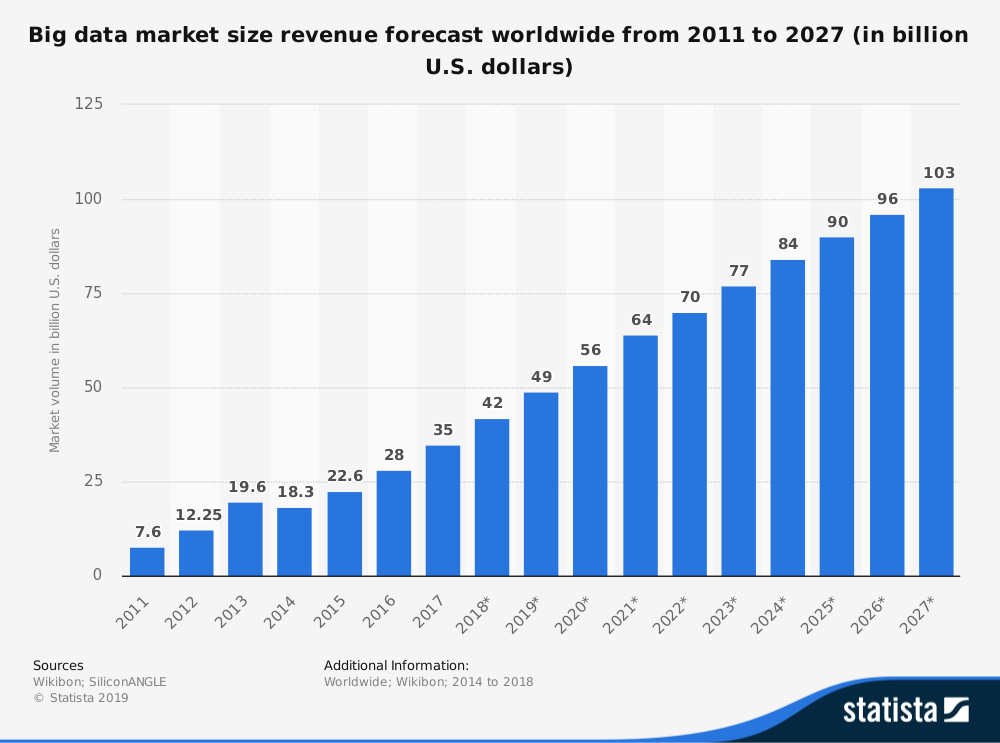
\includegraphics[scale=0.5]{revenue_forecast_statista}
    \caption{Forecast of Big Data market size, based on revenue, from 2011 to 2027 (in billion U.S. dollars) \cite{statista_market_forecast:online}}
    \label{fig:revenue_forecast}
  \end{figure}
  \end{appendices}
\end{document}
